\newgeometry{top=1in,bottom=1in,right=1in,left=1in}
\chapter*{Bilag 1: Danske Bank forside}
\thispagestyle{empty}
\setcounter{page}{1}
\begin{figure}[H]
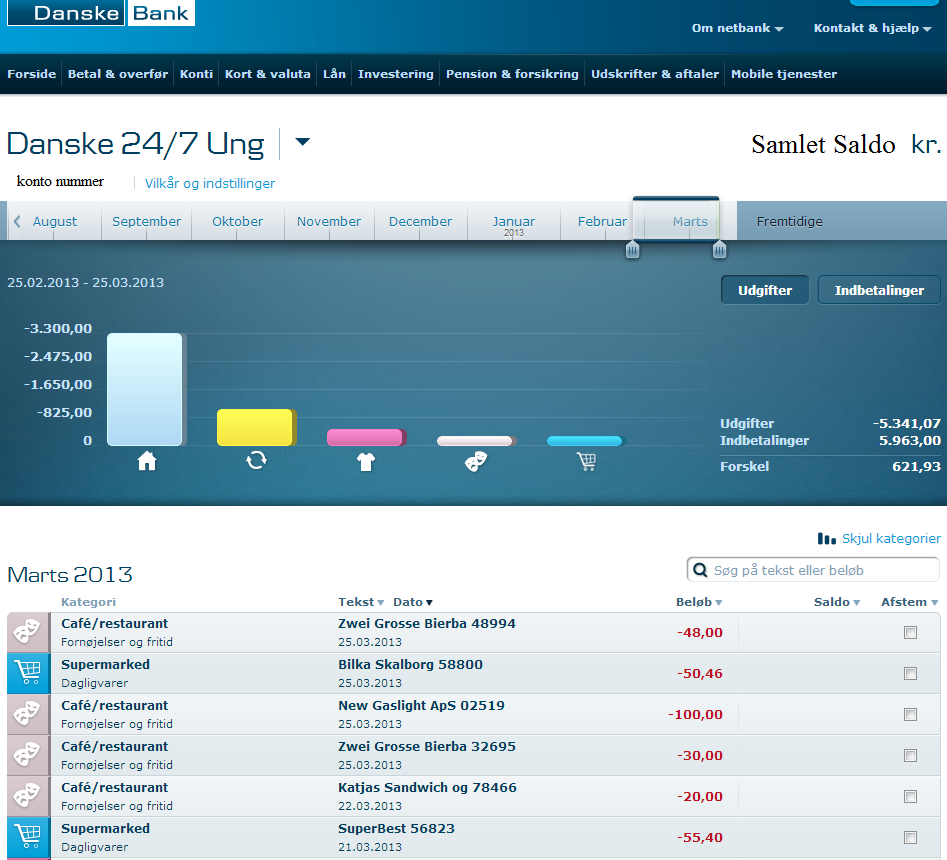
\includegraphics [width=\linewidth]{Billeder/bilagdb1.png}
\caption {Her ses et eksempel på den skærm man bliver mødt af når man logger ind på Danske Banks netbank}
\label {bilagdb1}
\end{figure}

\chapter*{Bilag 2: Databaseforbindelser}
\thispagestyle{empty}
\setcounter{page}{1}
\begin{lstlisting}[caption={Statisk klasse, der forbinder til objekt databasen NDatabase},label={lst:db}]
public static class db
{
	//En string dbFileName med filnavnet på databasen laves
	private const string dbFileName = "database.db";
	
	//Herefter åbnes database forbindelsen
	private static NDatabase.Api.IOdb odb = OdbFactory.Open(dbFileName);

	public static void Store(Transfer transfer)
	{
		//Objektet bliver sendt til databasen
		odb.Store(transfer);
		
		//Databasen bliver tvunget til at opdatere
		odb.Commit();
	}
	
	public static Collection<Transfer> GetTransfersForChild(Child child)
	{
		//Lav en LINQ forespørgsel
		var transfers = from transfer in odb.QueryAndExecute<Transfer>()
						where transfer.Recipient != null && transfer.Recipient.FullName == child.FullName
						select transfer;

		//Lav en collection til at indeholde Transfers
		Collection<Transfer> Transfers = new Collection<Transfer>();

		//Flyt alle Transfers objekter fra transfers til Transfers (sikrer at forespørgslen bliver udført)
		foreach (var t in transfers)
			Transfers.Add(t);

		return Transfers;
	}
}
\end{lstlisting}
\vspace{1cm}
\begin{lstlisting}[caption={Statisk klasse, der forbinder til den relationelle database SQLite},label={lst:sqlite}]
public static class db
{
	//Navnet på filen databasen skal gemmes i
	private const string dbFileName = "test.sqlite";
	private static SQLiteConnection conn;

	//Metoder til at åbne og lukke forbindelsen til databasen
	public static void OpenDB()
	{
		conn = new SQLiteConnection("Data Source=" + dbFileName + ";Version=3;");
		conn.Open();
	}
	public static void CloseDB()
	{
		conn.Close();
	}

	public static void Store(Transfer transfer)
	{
		//Få fat i ID'et på Recipient 
		int ChildIDInDB = GetIDOfChild(transfer.Recipient);
		string ChildID = ((ChildIDInDB == 0) ? "null" : ChildIDInDB.ToString());

		//Selve SQL forespørgslen bliver lavet som en streng
		string query = "INSERT INTO Transfers (Title, Description, Amount, Recipient, Date, Type, Sender) VALUES ('" +
						transfer.Title + "', '" +
						transfer.Description + "', '" +
						transfer.Amount.ToString(CultureInfo.GetCultureInfo("en-GB")) + "', '" +
						ChildID + "', '" +
						SQLiteConvert.ToUnixEpoch((DateTime)transfer.TransferDate) + "', '" +
						//DateTimeToUnixTimeStamp((DateTime)transfer.TransferDate) + "', '" +
						(int)transfer.Type + "', '" +
						GetIDOfUser(transfer.Sender) + "')";
						
		//SQL kommandoen bliver udført
		SQLiteCommand command = new SQLiteCommand(query, conn);
		command.ExecuteNonQuery();
		NotifyTransferCreated(transfer);
	}

	//Metode der tager mod et objekt af typen Child, og returnerer Transfers
	public static Collection<Transfer> GetTransfersForChild(Child child)
	{
		//En SQL kommando opbygges
		string query = "SELECT * FROM Transfers WHERE " +
						"Recipient IN (SELECT ID FROM Childs WHERE " +
						"FirstName='" + child.FirstName + "'" +
						")";

		//Kommandoen udføres
		SQLiteCommand command = new SQLiteCommand(query, conn);
		SQLiteDataReader r = command.ExecuteReader();

		Collection<Transfer> TransferList = new Collection<Transfer>();

		//For hvert række returneret af databasen
		while (r.Read())
		{
			int ID = r.GetInt32(r.GetOrdinal("ID"));
			string Title = r.GetString(r.GetOrdinal("Title"));
			string Description = r.GetString(r.GetOrdinal("Description"));
			decimal Amount = r.GetDecimal(r.GetOrdinal("Amount"));
			Child Recipient = child;
			DateTime Date = SQLiteConvert.ToDateTime(((long)r["Date"]).ToString(), SQLiteDateFormats.UnixEpoch, DateTimeKind.Local);
			ActivityType Type = (ActivityType)(long)r["Type"];
			User Sender = ((long)r["Sender"] == 0) ? null : GetUser(r.GetInt32(r.GetOrdinal("Sender")));

		//Lav et nyt objekt af typen Transfer, og tilføj det til TransferList
		TransferList.Add(new Transfer(Title, Description, Amount, Recipient, Date, Type, Sender));
	}

	return TransferList;
}
\end{lstlisting}